% 1977 年新疆卷（文科）第七题：直线 y=-x-3 过 B(-3,0) 与 A(2,-5) 的坐标系示意图，
% 两轴带箭头，坐标轴上绘单位刻度点（按源卷第 5 页布局）
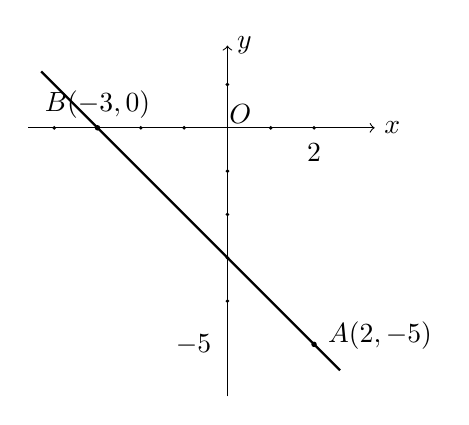
\begin{tikzpicture}[scale=0.55]
  \draw[->] (-4.6,0)--(3.4,0) node[right] {$x$};
  \draw[->] (0,-6.2)--(0,1.9) node[right] {$y$};
  \node at (0.30,0.32) {$O$};
  % 单位刻度点
  \foreach \xx in {-4,-2,-1,1,2} \fill (\xx,0) circle (1.3pt);
  \foreach \yy in {1,-1,-2,-3,-4} \fill (0,\yy) circle (1.3pt);
  \node[below] at (2,-0.15) {$2$};
  \node[left] at (-0.15,-5) {$-5$};
  % 直线 y=-x-3
  \draw[thick] (-4.3,1.3)--(2.6,-5.6);
  \fill (-3,0) circle (1.8pt) node[above] {$B(-3,0)$};
  \fill (2,-5) circle (1.8pt);
  \node[right] at (2.1,-4.8) {$A(2,-5)$};
\end{tikzpicture}
